% !Mode:: "TeX:UTF-8"
\chapter{限制分支预测宽度的设计}

本章首先介绍香山雁栖湖架构的取指策略,接下来介绍在高性能处理器中,按照指令地址对齐的取指策略,和不对齐的取指策略的优缺点。并指出为什么需要限制分支预测的宽度,过宽的分支预测宽度会对处理器整体设计带来怎样的影响。最后介绍在南湖架构中,修改取指策略,限制分支预测宽度相关技术的实现。具体有FTB表项的数据结构设计,以及FTB更新和管理策略,并解释了为什么要这样设计。通过修改每拍取指的基本单位,实现了限制前端在一次取指内容中分支指令的上限。

\section{香山雁栖湖架构取指策略}

在不同的处理器中,有许多种取指策略。例如在香山雁栖湖架构的设计中,取指PC是按照32Bytes对齐的,也就是低5位都为0,每次取指固定取32Bytes的指令数据。这种对齐取指设计好处在于可以有效避免在一次取指中指令跨Cache行的情况,取指单元每次取指只需访问一个Cache行。而这一点在南湖架构的设计中已被修改,南湖架构的取指单元在每次取指时最多可以同时取出2个Cache行的数据。其次就是由于指令都是对齐的,因此一条指令在整个取指的block中的位置是固定的,由低5位决定。这样可以保证在进行分支预测时,每条分支指令都只会被预测器的同一个bank预测、记录和更新,不会出现同一条指令在不同bank的情况。而南湖架构的设计中的取指不再对齐,也因此有可能出现同一条分支指令保存在不同的表项中的情况,这在某种程度上会降低预测器存储空间的使用效率。

但是按照指令地址对齐取指也有一些弊端,首先如果某次取指的起始PC非常靠近其所在的Cache行的末尾,由于取指单元不能够跨Cache行取指,则这次取回的有效指令数量就不满32Bytes,一定程度上会降低取指的带宽。其次,也是决定在南湖架构中修改这个机制的最主要的原因,即由于香山实现了RISC-V的C扩展,压缩指令集,RISC-V正常的一条指令 (RVI) 占4个Bytes,而C扩展中规定了许多压缩指令 (RVC),这些压缩指令只有2个Bytes长。增加了压缩指令之后,会带来一些问题,首先即使取指是按照32Bytes对齐,仍然会出现需要跨行取指的情况,如图\ref{fig:figure31}所示,为便于表示,以一个cache行 8Bytes为例,实际设计中一个cache行会大得多。图\ref{fig:figure31}(a)是不带压缩指令的情况,所有指令都是对齐的,不会出现一条指令在两个cache行中各存一半的现象,但是加入了压缩指令之后就会出现图\ref{fig:figure31}(b)的这种情况,即由于加入了压缩指令,非压缩的指令无法对齐,就会出现一条非压缩指令被2个相邻的cache行截断的情况。这种情况不光适用于RISC-V架构的处理器,所有使用有压缩指令定义的指令集架构的处理器都会有类似的问题。

当出现这种情况时,就会导致最后这条分支指令无法在一个周期内被完整取出,如果这条被截断的指令正好是条分支,便只能等到下一周期取到后半条指令码后再进行预译码操作。

\begin{figure}[htb]
    \centering
    \setlength\tabcolsep{3pt}  % 同一行中的图片间隔
    \vspace{5pt} % 图片上部的空白,如果太小的话,图片顶部会与正文内容十分接近
    \begin{tabular}{ccc}
        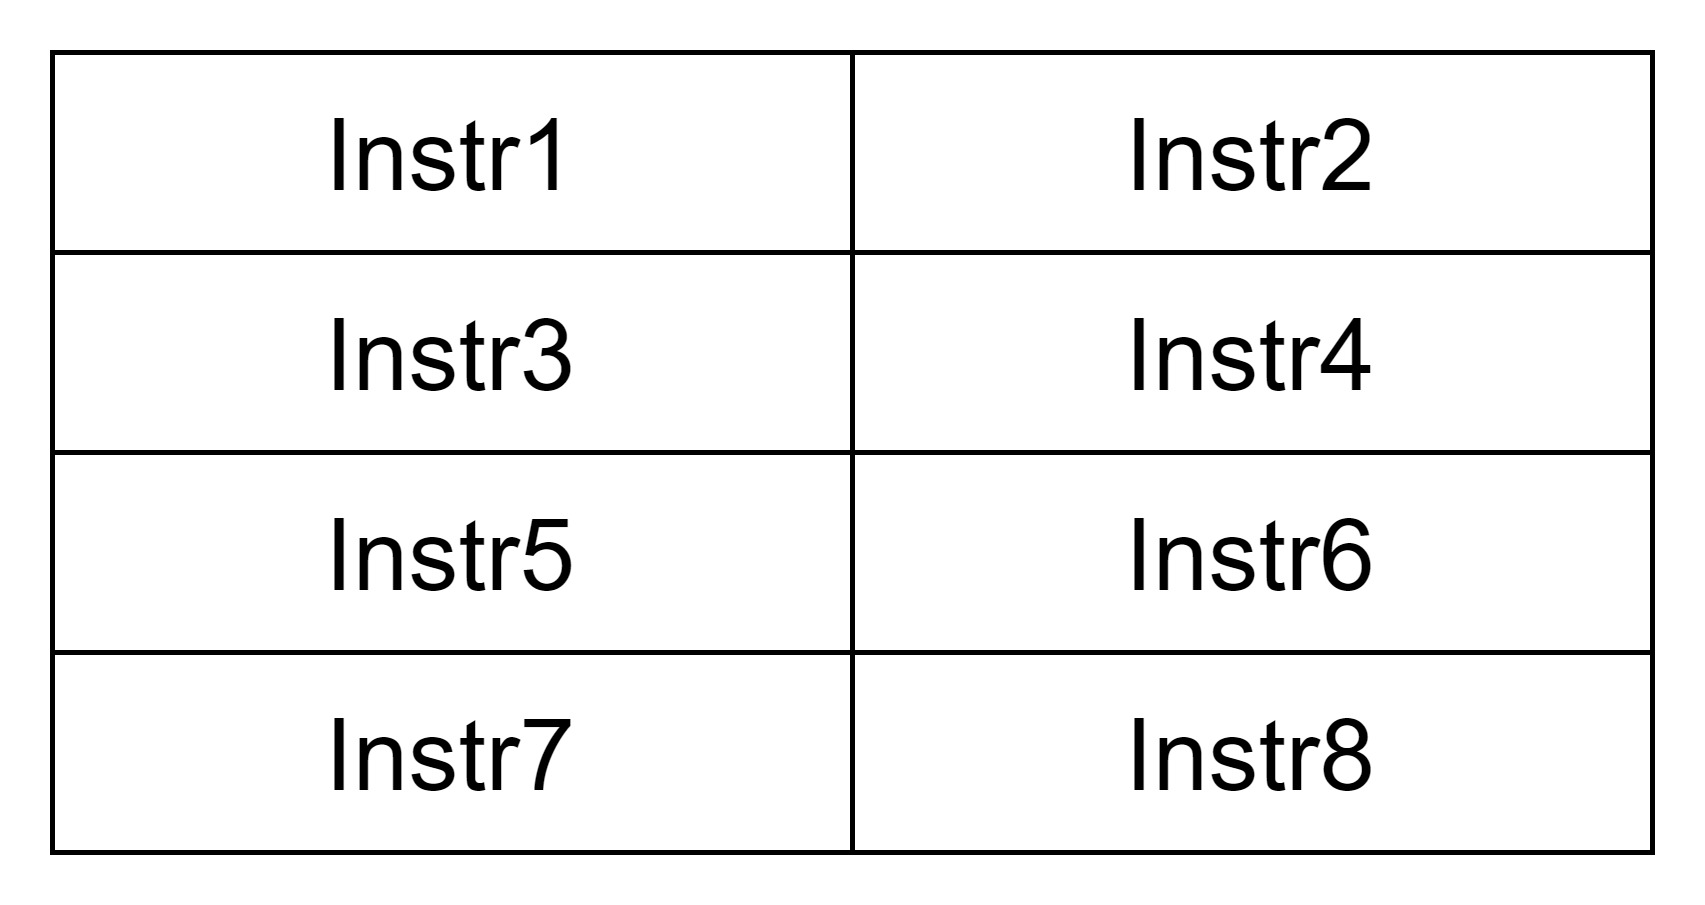
\includegraphics[width=0.30\textwidth]{RVI-only.jpg} &
        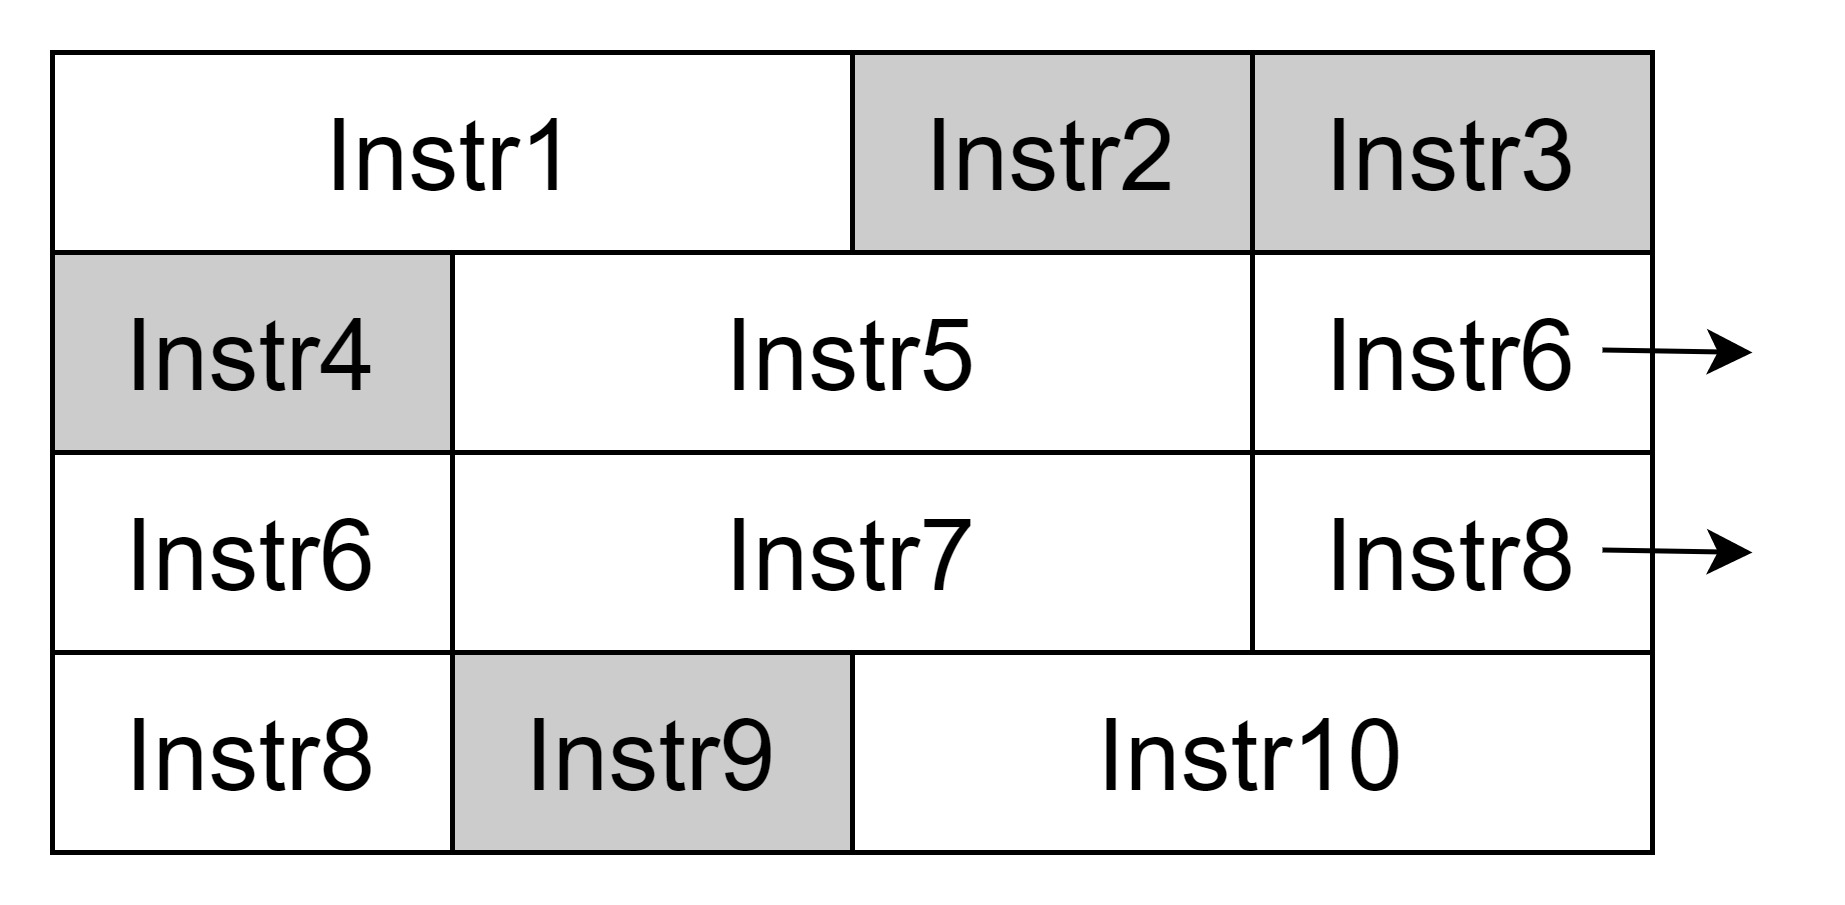
\includegraphics[width=0.325\textwidth]{RVIC.jpg} &
        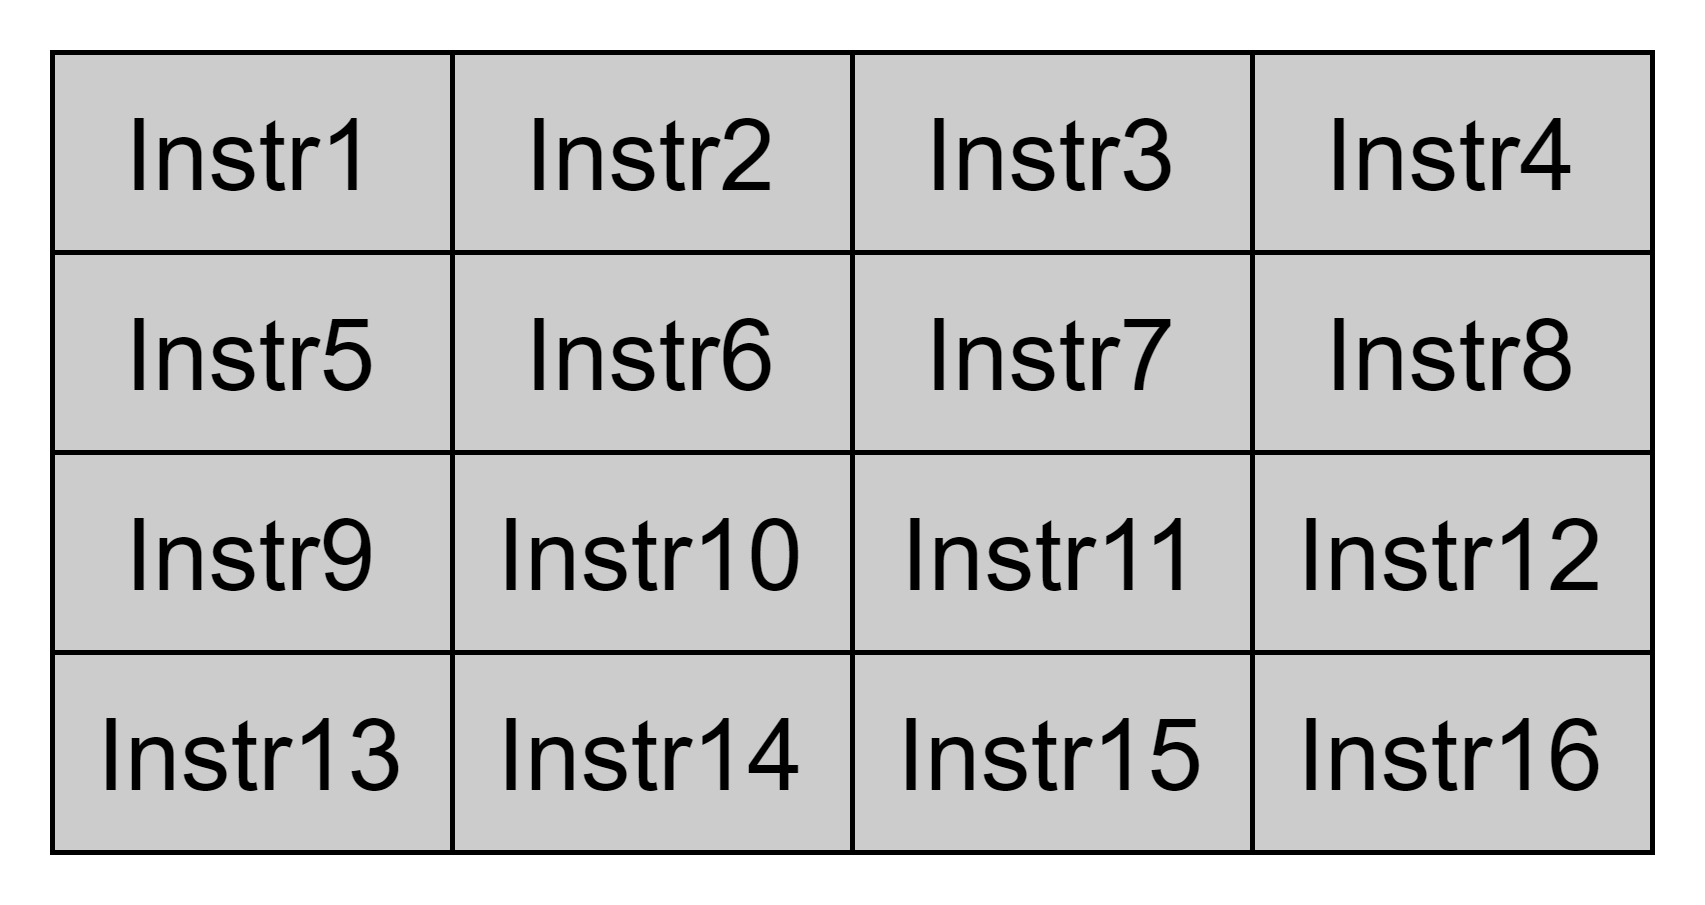
\includegraphics[width=0.30\textwidth]{RVC-only.jpg} \\
        (a) 只有RVI指令 & (b) RVI,RVC指令混合 & (c) 只有RVC指令 \\[1ex]
    \end{tabular}
    \caption{在cache行中以不同形式储存的指令码,其中白色的代表非压缩指令RVI,灰色的代表压缩指令RVC,图(b)中第6和第8条指令出现跨cache行情况}
    \label{fig:figure31}
\end{figure}

加入了压缩指令之后,如果以32Bytes为单位取指,每次取出来的数据中会有8到16条指令不等,最多的情况如图\ref{fig:figure31}(c)所示,即16条都是压缩指令的情况。因此为了能够覆盖到所有情况,香山雁栖湖架构的分支预测设计中,所有的预测器,包括雁栖湖架构中FTB的原型BTB (Branch Target Buffer) 都是以16为宽度来设计的,也就是说每个预测器都有16个bank,每个bank对应32Bytes中所有有可能是一条分支的位置。

但实际上真正在程序运行中,一次取出的指令中有这么多条分支指令的情况非常少见,这种设计在一定程度上是冗余的,意味着所有的分支预测逻辑的连线和复杂度都会大大增加,尤其是在分支预测决定最终的预测结果,给出下一周期需要预测的PC的时候,需要从预测器16个bank的预测结果中选出一条最终预测跳转的分支,从16个备选的跳转目标地址中选出一个最终的地址,这是一个4级的多选操作,而这个逻辑处于整个分支预测的关键路径上,许多的组合逻辑电路都要经过这段逻辑,因此降低分支预测宽度,能够减少分支预测的组合逻辑复杂度,减少选择最终预测结果的逻辑门数,如图\ref{fig:figure33}所示,最终达到优化时序,提高频率的效果。

根据开发过程中实际的时序报告来看,通常一个选择逻辑门MUX的时延在15ps左右,通过减少选择逻辑的层数,可以降低约45ps左右的时延,而整体频率要求所有的路径时延在350-400ps左右。但因为南湖架构相比于雁栖湖架构分支预测整体的改动很大,很多路径的变化也很大,减少选择逻辑的同时也新增了其他的逻辑。因此实际效果并不会如此直观。

除了香山处理器外,在IBM zEC12\cite{ibm-zec12},龙芯\cite{loongson}等公司的商业处理器的相关论文和文档中都提到了有限制分支指令最大数量的相关技术,是目前高性能处理器领域的一个主流趋势。

\begin{figure}[htb]
	\centering
	\setlength\tabcolsep{3pt}  % 同一行中的图片间隔
	\vspace{5pt} % 图片上部的空白,如果太小的话,图片顶部会与正文内容十分接近
	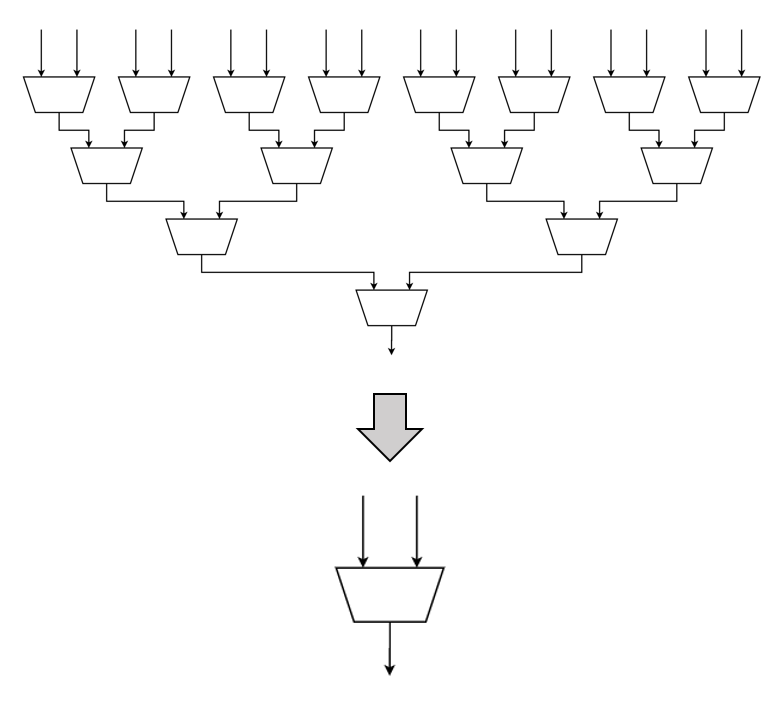
\includegraphics[width=0.7\textwidth]{mux.png}
	\caption{降低分支预测宽度后,选择最终生效分支指令的选择逻辑门层数变少}
	\label{fig:figure33}
\end{figure}

\section{Fetch Block的定义}

为降低分支预测宽度,一个思路是限制每次取指所能包含的分支指令的最大数量,因为分支预测最终的宽度是以可能的最大分支数量为准,例如上文提到的如果一次最多会有16条分支,那么分支预测宽度也必须为16,即使大部分时候并没有这么多分支。
假设将分支预测的宽度限制为2,之前的取指是以32Bytes定长为单位取指的,而在一些分支指令密集的程序片段中,32Bytes大小的指令块中大概率会出现超过2条分支,因此不能够继续以固定的大小作为取指的基本单位,需要定义一个新的基本单位,为这个单位添加一些约束条件,以此来限制每次取指的分支指令数量。

在南湖架构的分支预测架构中,定义了Fetch Block,这个概念是Glenn\cite{scalable-frontend}提出的,Fetch Block的定义如下,每个block都必须满足这三个约束条件:

\begin{enumerate}
    \item 每个block的最大大小为32Bytes,即当一段指令中没有分支指令时,仍然需要限制block的最大大小,因此规定block的最大大小和雁栖湖架构相同,都是32Bytes。
    \item 当遇到第n+1条条件跳转指令 (branch) 时,无论block大小有没有32Bytes,这个block在第n+1条branch指令之前截止。为什么不是在第n条指令后就立即截止,是因为这样就可以保证,在block中最多只有n条分支的前提下,每个block中的指令数量尽可能多。
    \item 当遇到无条件跳转指令 (jump) 时,无论block大小有没有32Bytes或有没有达到n条branch指令的上限,这个block都在这条jump指令后截止。这是因为jump指令必然是跳转的,因此在这条指令之后下一周期需要预测的PC应该由预测器给出,无论下一周期从哪里开始预测,都将会是另一个block。因此如果block中含有jump指令,必定是block中最后一条指令。
\end{enumerate}

通过以上的3条约束,就能够保证单个的Fetch Block中,branch指令不超过n条,且最多只有一条jump指令。而在此基础上,本文又提出了一种改进策略,可以略微减少FTB表项的大小,节省一些面积。将每个block中看作有n个装branch指令的slot和1个装jump指令的slot,假设因为遇到第n+1条指令导致block截止时,其中存储jump的slot就被闲置了;而遇到jump指令,且之前不足n条branch指令时,第n条branch指令的slot也被闲置了,而这两种情况非常常见,带来了空间的浪费。可以针对这种现象做出改进,即令第n条branch指令与jump指令共用一个slot,即在block中的最后一个slot既可以用于存储一条branch指令的信息,也可以用于存储一条jump指令的信息。这样一个block中就变为最多可以同时有n条branch指令,或者同时有n-1条branch指令和1条jump指令。

通过Fetch Block的定义不难发现,Fetch Block是不可能按照地址对齐的。因此同一条分支存在于两个不同的Fetch Block中是有可能的,而这种情况会带来一定的存储空间浪费,经过测试,在使用相同SRAM开销的情况下,以Fetch Block为表项存储FTB的命中率是略低于以分支指令为表项存储的BTB的命中率的。因此南湖架构中增加了FTB使用的SRAM大小。此外一个block中的指令跨Cache行也是有很大概率出现的情况,因此在南湖架构的设计中,取指单元每次取指可以取出2个Cache行,以保证每个block都能在一次指令缓存访问中取出。

\section{FTB的数据结构设计}

% 投稿论文的主要内容

为了在硬件中实现以Fetch Block为表项的FTB,本文设计了一种FTB表项的数据结构,相关的属性以及作用在表\ref{tb:table1}中列出。通过这些属性,就能够清楚的描述一个Fetch Block的状态,以及其中含有的分支指令的相关信息。

\begin{table}[]
	\caption{FTB表项属性列表}
	\label{tb:table1}
	\centering
    \begin{tabular}{ccc}
        \toprule
        属性名 & 数据类型 & 含义及作用 \\
        \midrule
        valid & Bool & 代表这个表项是否有效 \\
		tag & Unsigned Int & Fetch Block起始地址的高位 \\
		brSlots & Vector(FtbSlot) & 用来存储branch指令的信息,FtbSlot的定义见表\ref{tb:table2} \\
		tailSLot & FtbSlot & 用来存储branch/jump指令的信息 \\
		pftAddr & Unsigned Int & \tabincell{c}{代表这个block最后一条指令的下一条指令的起始PC, \\ 存储低位,使用拼位计算} \\
		carry & Bool & 代表拼位计算时高位要不要加1 \\
		isCall & Bool & 如果block中有jump时,代表这条jump是否是call指令 \\
		isRet & Bool & 如果block中有jump时,代表这条jump是否是ret指令 \\
		isJalr & Bool & 如果block中有jump时,代表这条jump是否是jalr指令 \\
		last\_may\_be\_rvi\_call & Bool & 最后一条指令可能是半条RVI Call指令 \\
		always\_taken & Vector(Bool) & 这条指令是否总是跳转 \\
        \bottomrule
    \end{tabular}
\end{table}

从表\ref{tb:table1}中可以看出,在FTB表项中,存储了Fetch Block的tag,分支指令的相关信息,以及计算Fetch Block结束地址的相关信息。其中的brSlots和tailSlot是用来存储block中的branch和jump指令信息的,它们是同一种数据结构FtbSlot,不同之处在于brSlots是一个有n-1个FtbSlot的列表,而tailSlot就是一个单独的FtbSlot。FtbSlot的相关属性以及作用在表\ref{tb:table2}中列出。

% \begin{table}[]
% 	\caption{FtbSlot属性列表}
% 	\label{tb:table2}
% 	\centering
% 	\begin{tabular}{|c|c|c|}
% 		\hline
% 		属性名   & 数据类型   & 含义及作用   \\ \hline
% 		valid & Bool & 这条branch/jump是否有效 \\ \hline
% 		offset & Unsigned Int & 这条branch/jump指令在block中的offset \\ \hline
% 		lower & Unsigned Int & \tabincell{c}{这条branch/jump的target的低位, \\ branch和jump的offset length是不同的} \\ \hline
% 		tarStat & Unsigned Int & \tabincell{c}{这条branch/jump指令的目标地址高位是需要加1或者减1或者不变, \\ 0代表不变,1代表加1,2代表减1} \\ \hline
% 		sharing & Bool & 这个slot现在存的是一个branch还是一个jump \\ \hline
% 	\end{tabular}
% \end{table}

\begin{table}[]
	\caption{FtbSlot属性列表}
	\label{tb:table2}
	\centering
    \begin{tabular}{ccc}
        \toprule
        属性名 & 数据类型 & 含义及作用 \\
        \midrule
        valid & Bool & 这条branch/jump是否有效 \\
		offset & Unsigned Int & 这条branch/jump指令在block中的offset \\
		lower & Unsigned Int & \tabincell{c}{这条branch/jump的target的低位, \\ branch和jump的offset length是不同的} \\
		tarStat & Unsigned Int & \tabincell{c}{这条branch/jump指令的目标地址高位是需要加1或者减1或者不变, \\ 0代表不变,1代表加1,2代表减1} \\
		sharing & Bool & 这个slot现在存的是一个branch还是一个jump \\
        \bottomrule
    \end{tabular}
\end{table}

一个Fetch Block的起始地址就是block中第一条指令的PC,而block的结束地址应该是block中最后一条指令的PC。但由于指令分为4Bytes的RVI指令和2Bytes的RVC指令,所以只存储block中最后一条指令的PC,并无法知道最后一条指令的长度是4Bytes还是2Bytes,也无法推断出这个Fetch Block后面连续的Fetch Block的起始地址,因此需要存储下一个顺序Fetch Block的起始地址,称为fallthrough address。而完整的fallthrough address可以通过起始地址和pftAddr (partial fallthrough address) 以及carry属性计算得到。由于一个Fetch Block最大的大小不超过32Bytes,以香山举例,完整的指令地址有39位,通常来说一个Fetch Block的起始地址和结束地址的高34位要么是相同的,要么结束地址的高34位是起始地址的高34位加1。因此没有必要存储完整的fallthrough address,只需要存储fallthrough address的低5位,以及它的高位是否需要由起始地址加1得到即可,在计算fallthrough address时只需要使用block起始地址的高34位 + carry,再与pftAddr拼接,即可得到39位的完整fallthrough address。

而FtbSlot中的lower和tarStat类似于pftAddr和carry,不同之处在于分支指令的跳转距离不止32Bytes,因此lower的位数等于指令码中用于计算偏移地址的offset字段的位数,且由于jump指令的offset字段和branch指令的offset字段位宽不同,brSlots和tialSlot中lower的位宽也不同。同时由于分支指令既可以向前跳转,又可以向后跳转,所以分支指令的跳转目标地址高位有3种可能:与block的起始地址相同、起始地址加1、起始地址减1。所以tarStat需要2bit位宽,可以表示0、1、-1三种情况。需要计算某条分支的跳转目标地址时,也是将起始地址的高位加上tarStat,再与lower拼接得到完整的目标地址。

isCall和isRet属性主要用于标记哪些分支需要使用RAS进行预测。isJalr用于标记哪些分支是间接跳转分支指令,需要使用ITTAGE预测器预测。

always\_taken是对于一些固定跳转分支的优化,一条分支只有在至少一次跳转之后,才会被认作有效的分支加入FTB中,而一条刚加入FTB的分支会为它标记为always taken,之后无论预测器预测结果如何,都会预测这条分支是跳转的,如果这条分支之后有一次不跳转,always taken标志就会被消除。

\section{FTB的管理策略}

在雁栖湖架构BTB设计中,每次有指令提交后,如果其中有分支指令,就会在BTB中找到分支指令PC对应的表项,选择一个空闲的way写入,如果所有的way都已经被占用,就使用随机替换方式,替换已有的一个表项。而由于在南湖架构中使用了以Fetch Block为基本单位的FTB,并且计划将其替换策略更改为PLRU (伪最近最少使用, Pseudo-Least Recently Used)算法,因此FTB的管理策略有较大的改动。

在FTB的设计中,由于限制了每个Fetch Block中分支指令的最大数量,因此大部分时候一个block中的有效数据是小于32Bytes的,这一定程度上会导致FTB的存储空间使用效率不高。为了尽可能增大每个Fetch Block中有效指令的数量,在新建Fetch Block时先将所有未跳转过的分支指令都看作普通的指令,只有跳转过的分支才会被记录到FTB中,而实际上,在程序中一些一直不跳转的分支指令也占有一定的比例,如此便可以直接忽略这类分支指令。而这种策略就导致了随着越来越多的分支指令跳转之后,每个Fetch Block的大小,其中分支指令的分布情况,在程序执行过程中是动态改变的,需要有一个完善的策略,针对不同的情况对FTB中的相关信息进行维护。

经过分析可以将FTB表项的更新分为以下几种情况:

\begin{enumerate}
	\item 在最开始时,FTB为空,因此所有的分支指令都识别不出来,默认都是不跳转,所以最初的所有Fetch Block都是32Bytes,且其中视为没有任何分支指令。
	\item 在一次指令提交中,原有的block中检测到了新的branch指令,而block中的branch指令数量没有达到上限,还有多余的slot时,将新的branch指令插入到这个block中。
	\item 在一次指令提交中,有新的branch指令加入,但block中已经没有多余的slot时,需要对比新的branch指令和block中已有branch指令的先后关系,取前n条branch指令按顺序加入到block中,n代表当前block中所能够存储的branch指令的最大值。剩余的一条branch指令需要从block中去除。
	\item jump指令不存在不跳转的情况,因此一定是在新建block的时候加入到存放jump的slot中,而如果是共享slot的话,如果有新的branch指令,它的PC在jump指令之前,就需要将jump挤出该block,branch指令存入共享的slot中,这条jump指令之后会被加入到一个新建的block中。
\end{enumerate}

% 这里的逻辑有空再理一理

无论是上面的哪一种情况,除了需要根据不同的情况调整slot中的数据,由于最后一条分支可能会改变,因此还需要修改block的fallthrough address。图\ref{fig:figure32}画出了不同情况下需要做的操作。首先需要看这条新的branch指令能否插入到block中,如果不能,说明所有的slot都满了,且它们的指令序都在这条新的branch指令之前,所以根据Fetch Block的定义,block在第n+1条branch指令之前截止,且这条指令的PC和block的起始地址之间不超过32Bytes的大小要求,则需要将fallthrough address修改为这条新的branch指令的PC。而如果这条branch指令能够插入,且没有分支指令被替换出block,则fallthrough address可以保持不变。如果有分支指令被替换出block,无论是branch指令还是jump指令,都将fallthrough address设为被替换出block的指令的PC。

\begin{figure}[htb]
	\centering
	\setlength\tabcolsep{3pt}  % 同一行中的图片间隔
	\vspace{5pt} % 图片上部的空白,如果太小的话,图片顶部会与正文内容十分接近
	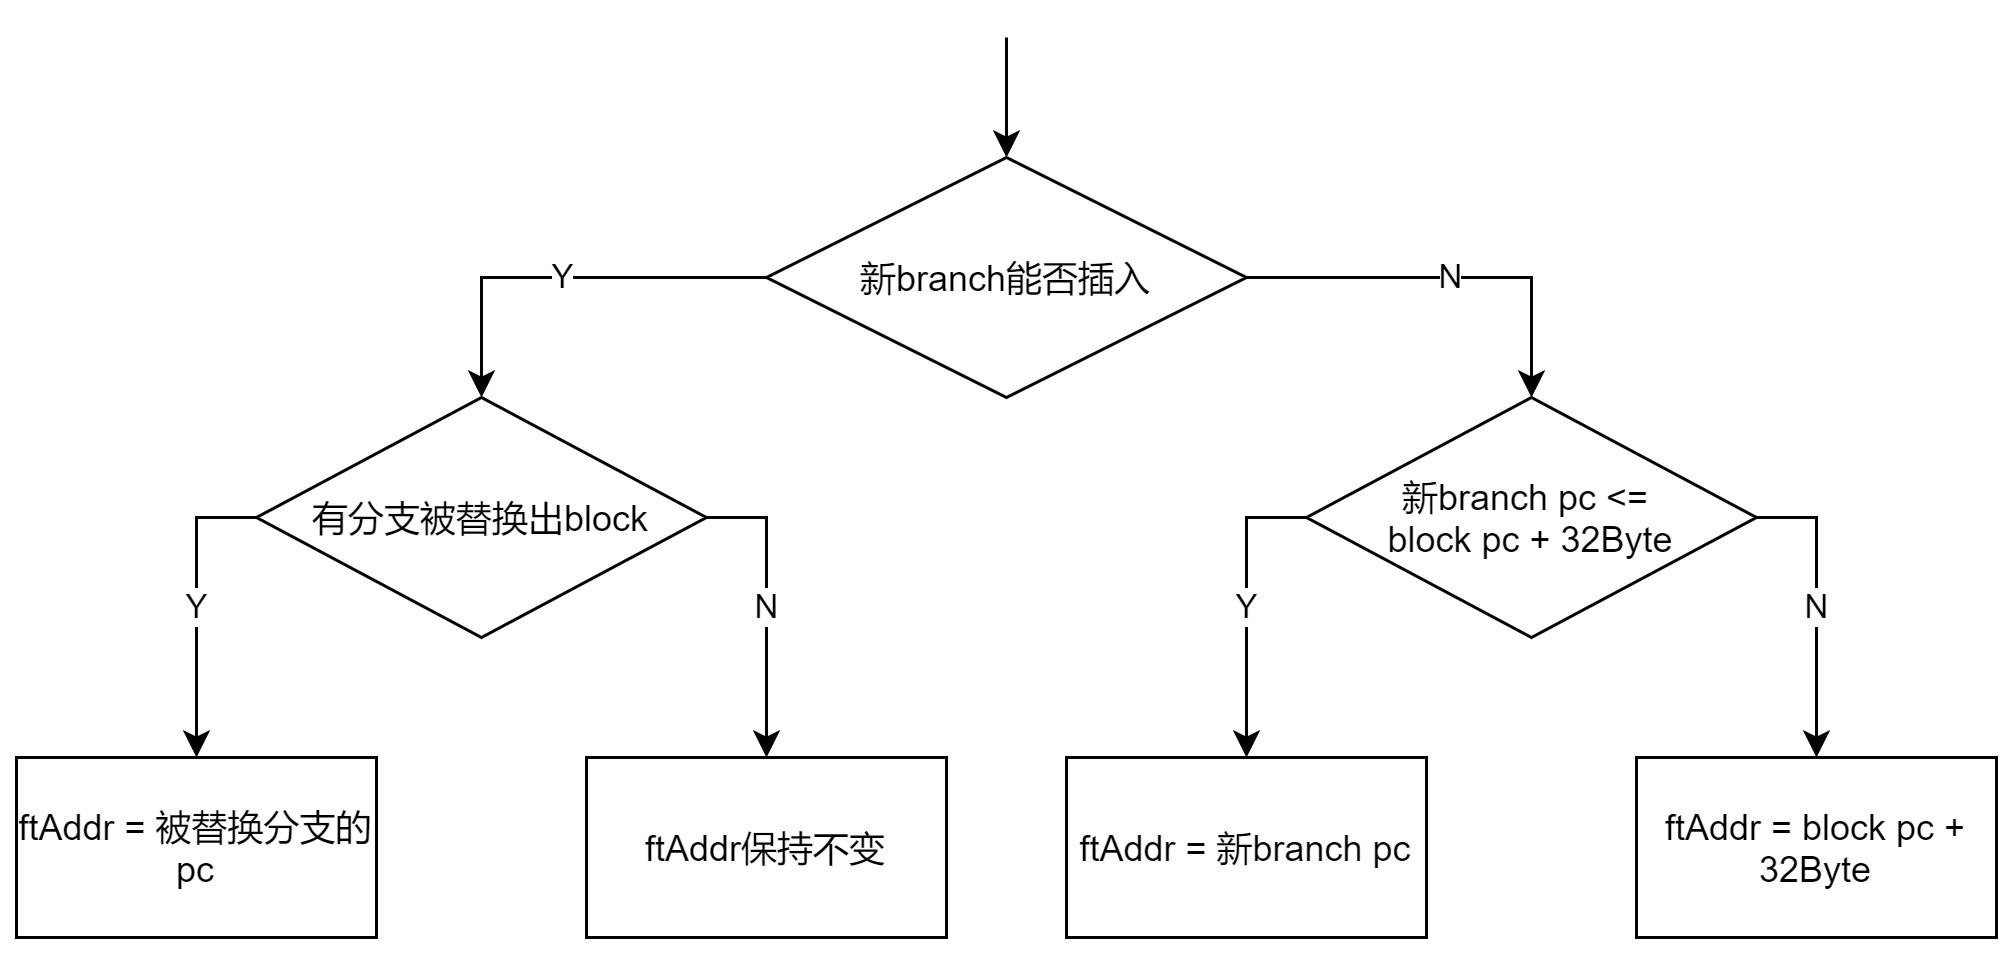
\includegraphics[width=1\textwidth]{ftb-manage.jpg}
	\caption{FTB更新时Fetch Block fallthrought address的变化,ftAddr表示fallthrough address}
	\label{fig:figure32}
\end{figure}

除了维护已有的Fetch Block,如果有新的block需要写入FTB,但是对应的way已满,则需要选择其中一个block替换出去,在雁栖湖架构中BTB使用的是随机替换策略,在南湖架构中改为PLRU替换策略,并且使用的是用Chisel实现的通用替换策略模块,可以非常快速灵活的更改替换策略,在香山的各级缓存中使用的也是相同模块。

写入新的block时需要注意,如果这个block已经在FTB中存在,那么只需要更新其中的block即可,而不能够写入两个起始地址相同的block,这样会导致查找FTB时出现多路命中 (multiple hit) 的错误,这会影响到FTB中存储信息的正确性,从而影响分支预测的性能。因此,在添加或者替换block之前,首先需要确认这个block是否已经存在于FTB之中。最直观的方法就是查找一次FTB,就可以知道block是否已经存在,但是由于FTB是使用单口SRAM来存储主要数据的,一个周期内只能够读或者写,因此在添加或替换FTB时,首先需要阻塞分支预测流水线,因为分支预测也需要读FTB来获取分支相关的信息。之后再花一个周期先读FTB,检查block是否已经在FTB中,如果已经存在,在哪一个way中,如果不存在,则给它分配一个way,下一周期再写入FTB。这样一来,每次添加或替换FTB时,预测流水线都会堵塞2个时钟周期。这会导致预测效率的降低,为此本文做了以下两点优化,能够减少大部分指令提交时的FTB读需求:

\begin{enumerate}
	\item 在预测时会将当前预测的block是否在FTB中命中,以及哪一way命中的信息,作为FTB预测的meta信息传入FTQ中保存,而在这个block中的指令提交时,FTQ会将这个命中信号传回FTB,如果在预测时这个block就已经存在于FTB中了,那么在指令提交时这个block大概率仍然存在于FTB中,并且即使在这段时间内这个block被替换出FTB了,也依然不会出现multiple hit的情况。如果发现预测时这个block就已经在FTB中命中。只要直接将更新后的block写入预测时保存的那个way中即可,不用再查找一次FTB。当然如果没有命中,仍然还是要查找一次FTB。通常FTB的命中率很高,使用这种策略能够减少大量不必要的堵塞。
	\item 在试图更新block时,会检测block在这次提交中是否有新的分支,其中的信息是否有改动,如果这次提交没有给原有的block带来任何改动,那么就不用写入FTB,避免没有意义的写入。
\end{enumerate}

通过以上两点优化,可以极大减少由于更新导致的FTB读写,降低对分支预测流水线的影响。经过测试,在做这两点优化前,在更新时先查找FTB会极大的降低分支预测流水线的预测效率,而优化后对分支预测的影响几乎没有。

% 相关的性能验证放在第5章写吧

\section{本章小结}

本章以香山雁栖湖架构中的32Bytes对齐取指开始讨论,阐述了对齐取指和非对齐取指的优劣,并给出了为什么在南湖架构中要修改对齐取指这一策略。提出了一种限制分支预测宽度的详细实现方案,主要包含FTB的详细设计,给出了FTB中用于存储Fetch Block的数据结构,并给出了在不同情况下Fetch Block更新时内部信息的管理策略,并提出了几种优化细节。最终将其应用在了香山处理器南湖架构的分支预测部件中。这种设计思路不仅可用于香山处理器,在其他的高性能处理器也可适用。通过使用FTB替换雁栖湖架构的BTB,并同时修改所有分支预测器的基本预测单位。分支预测的整体预测宽度从16缩减到了2,减少了分支预测关键路径上的逻辑电路延迟。并且整体前端分支预测与取指的带宽没有太大的损失。
